% !TeX root = Report.tex

\author{
    Joar Heimonen\\
    \texttt{contact@joar.me}
}

\documentclass[12pt]{article}
% include enumitem
\usepackage{enumitem}
\usepackage{listings}
\usepackage{sectsty}
\usepackage{color}
\usepackage{float}
\restylefloat{table}
\usepackage{graphicx}
\usepackage{biblatex}
\usepackage{tikz}
\usetikzlibrary{shapes, arrows.meta, positioning, shapes.geometric}
\usepackage{changepage}

\usepackage{xcolor}
\usepackage{listings}

\addbibresource{Library.bib}

\title{\textbf{PG3402 - Project Description} \\ A generic streaming service using microservices}
\date{\today}

\graphicspath{ {./images/} }

\begin{document}

\subsectionfont{\fontsize{12}{14}\selectfont}

\maketitle

\pagebreak

\tableofcontents



\section{Introduction}
This document will describe the implementation of a 
simple scalable streaming service built using multiple microservices \cite{Microservices2024}.
We will describe how the system handles user access control, content managment and load balancing.
The most important element of this project will be JSON web tokens\cite{jonesJSONWebToken2015} 
that allow data to pass between the different microservices. 
The service will also feature load balancing using the GoodDNS server\cite{heimonenSlenderman00GoodDns2023}.

\section{Overview} 
In this project, we aim to develop a robust streaming service that leverages a microservices architecture to offer 
scalable video streaming. The service is designed to cater to two main types of users: 
administrators and registered viewers. Administrators have the ability to upload and manage content, 
while registered users can browse and stream content.
The core functionalities include user registration and login, 
content management, and dynamic load balancing to handle varying loads. 
The system will utilize JSON web tokens for secure data transmission between 
microservices utilizing users as intermediates. 
it incorporate a custom DNS solution, 
GoodDNS \cite{heimonenSlenderman00GoodDns2023}, for load management.


%\section{Technical background}
%This section aims to describe the following terms:

\section{User Stories}

\subsection{Story 1: User Registration}
\textbf{As a} user, \\
\textbf{I want to} be able to register an account using a username and a password, \\
\textbf{So that} I can access the streaming service.

\begin{itemize}[label={}]
    \item \textbf{Acceptance Criteria:}
    \begin{enumerate}
        \item The registration screen is accessible from the home page.
        \item Users can enter a username and password.
        \item The system validates that the username is valid.
        \item An error message is displayed if the username is not valid.
    \end{enumerate}
\end{itemize}

\subsection{Story 2: Content Browser}
\textbf{As a} user, \\
\textbf{I want to} be able to browse content, \\
\textbf{So that} I can access and stream the content.

\begin{itemize}[label={}]
    \item \textbf{Acceptance Criteria:}
    \begin{enumerate}
        \item The homepage consists of a list of content.
        \item Users can select the content they want to watch.
        \item The system checks if the user is logged inn.
        \item The user is able to stream content when logged inn.
        \item A login prompt is shown if the user is not logged inn.
    \end{enumerate}
\end{itemize}

\subsection{Story 3: Add New Content}
\textbf{As an} Administrator, \\
\textbf{I want to} add new contet to the service, \\
\textbf{So that} users can watch the content.

\begin{itemize}[label={}]
    \item \textbf{Acceptance Criteria:}
    \begin{enumerate}
        \item There is an "Admin" button on the home page.
        \item Clicking the button takes the user to an admin page.
        \item The content can be submitted on the adming page.
        \item An error message is shown if the content submission fails.
    \end{enumerate}
\end{itemize}

\section{Requirements}
\subsection{Users}
The system must be able to handle user registration and login. 
This includes the ability to securely store user credentials and personal information in a database. 

\subsection{Content Management}
The system must be able to handle content uploading and streaming efficiently. 
This involves accepting new content from administrators, 
storing it in the content database and the file system, 
and serving it to authenticated users upon request. 
The system should support various media formats and ensure smooth streaming experiences even under high load. 
Additionally, content metadata management (like titles, descriptions, and tags) 
should be implemented to enhance content discoverability.

\subsection{Load Balancing}
The system should efficiently distribute incoming network traffic across multiple 
servers to ensure reliability and scalability. 
This involves using a DNS server that can dynamically allocate 
requests to the least loaded server. The load balancing DNS server
must have a second failover DNS server. If neceserry an infinite ammount of 
sub-sub DNS servers can be implemented. The time to live is used to control how often users poll the DNS servers for
new server allocations.

\begin{tabular}{c c}
~ ~ \textbf{ttl} & ~ ~ ~ ~ ~ \textbf{ttl} \\
~ ~ 0 & ~ ~ ~ ~ ~ 3600 \\
\end{tabular}

    
\begin{itemize}
    \item \texttt{userserver1.dns1.mydomain.com}
    \item \texttt{userserver1.dns2.mydomain.com}
    \item \texttt{contentserver2.dns2.mydomain.com}
\end{itemize}


\section{Architecture}

\subsection{Discussion}
There exists an almost infinite way to configure the nodes in our architecture. 
To avoid aquiring technical debt it is
of the upmost importance to derive an architecture fitting of our needs.
Therefor we have derived a simple set of architectural guidelines.

\begin{itemize}
    \item \textbf{Load Balancing}: The service must be able to efficiently balance load. No parts of the service can choke due to increased load.
    \item \textbf{Scalability}: All parts of the service must be able to scale as needed to account for increases in load.
    \item \textbf{Security}: The microservices must pass data to eachother in a secure manner.
    \item \textbf{Simplicity}: There should be no unnecesary complexity.
\end{itemize}

The simplest way for microservices to pass data to each other is trough the user in the form of
JSON web tokens. The following scenarios can be solved using both JSON web tokens and direct communication between the micro services.

\begin{itemize}
    \item \textbf{False metrics}: If metrics are not derived from the content management service but the client instead. False metrics might be reported by bad actors.
    \item \textbf{Non existing content IDs}: If content IDs in the metadata management services manifest is not derived from the content management service. Metadata might be created for content that does not exist.
\end{itemize}

\subsubsection{Load Balancing}
There are an infinte ammount of strategies for balancing load in services consisting of multiple nodes.
And there is much to be gained from utilizing lower level protocols to achieve this. Using GoodDNS solves
two problems, it lowers the bandwidth required as the DNS protocol as outlined in RFC 1035 is extremely light weight.
DNS also removes the need for proxying data allowing clients to communicate directly with the relevant services.
This makes for a much more reliable service as we don`t risk our proxying solution functioning as a bottleneck.

Using DNS also has a couple of drawbacks. The DNS system is complex and can be quite slow.
Recursive DNS servers not compliant with RFC 1035 might not respect a domains TTL.
In cases like these the service might break for users as they are feed out of date DNS data
from non-compliant DNS servers.

\subsection{Nodes}

\textit{Figure \ref{fig:AR}} shows a service consisting of the following microservices:

\begin{itemize}
    \item \textbf{DNS Server (Load Balancer)}: Directs incoming network traffic to different servers, 
    balancing the load and serving as a DNS resolver. All servers recieve their own sub-domains with short times to live.
    \item \textbf{Clients}: End-users who interact with the application through a web browser.
    \item \textbf{User Management Service}: Manages user authentication, authorization, and profiles, interfacing with the \textbf{User Database}.
    \item \textbf{Content Management Service}: Handles content storage and retrieval through the \textbf{Content Database} and manages file-based content with the \textbf{File System}.
    \item \textbf{Metadata Managment Service}: Handles the metadata related to content, this service consists of a manifest of all content that has been uploaded to the \textbf{Content Management Service}, content descriptions, titles and tags.
    \item \textbf{Metrics Service}: Keeps track of content views, likes and dislikes. 
    \item \textbf{Web Server}: Serves a static single page application used by the client to interact with the microservices.
    \item \textbf{Databases and File System}: Separate databases for users and content data ensure efficient management and scalability. The file system stores non-database content.
\end{itemize}

Communication between clients and services is secured using HTTPS, 
with REST API requests facilitating interactions between clients and microservices.
This architecture ensures security, and scalability under varying load.
\newline
\begin{figure}[h]

    \resizebox{15cm}{10cm}{%
        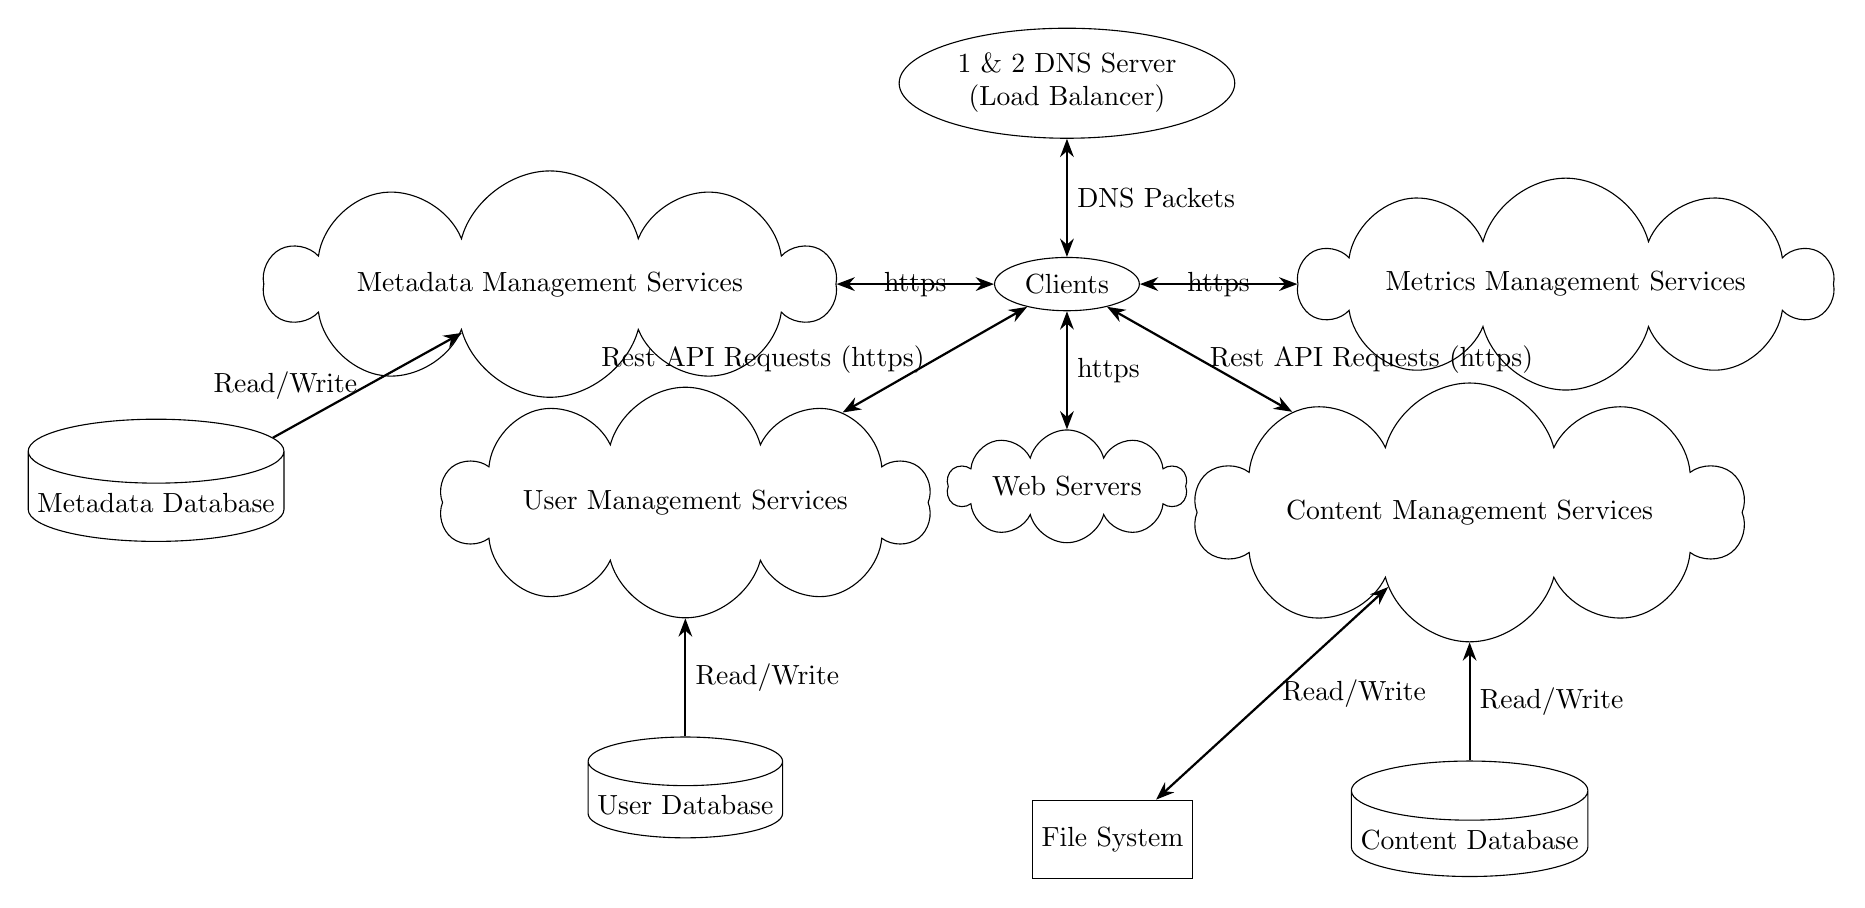
\begin{tikzpicture}[
            node distance=1.5cm and 2cm,
            mynode/.style={draw, ellipse, align=center},
            arrow1/.style={-Stealth, thick},
            arrow2/.style={Stealth-Stealth, thick},
            database/.style={draw, cylinder, shape border rotate=90, aspect=0.25, align=center},
            filesystem/.style={draw, rectangle, minimum width=2cm, minimum height=1cm, align=center},
        ]
        
            % Nodes
            \node[mynode] (dns) {1 \& 2 DNS Server\\(Load Balancer)};
            \node[mynode, below=of dns] (clients) {Clients};
            \node[cloud, aspect=4, draw, below left=of clients] (userLogin) {User Management Services};
            \node[cloud, aspect=4, draw, below right=of clients] (contentMgmt) {Content Management Services};
            \node[cloud, aspect=6, draw, left=of clients] (metaMgmt) {Metadata Management Services};
            \node[cloud, aspect=6, draw, right=of clients] (metricMgmt) {Metrics Management Services};
            \node[cloud, aspect=4, draw, below=of clients] (clientHost) {Web Servers};
            \node[database, below=of userLogin] (userDB) {User Database};
            \node[database, below=of contentMgmt] (contentDB) {Content Database};
            \node[database, left=of userLogin] (metaDB) {Metadata Database};
            \node[filesystem, left=of contentDB] (fileSystem) {File System};
        
            % Arrows
            \draw[arrow2] (dns) -- (clients) node[midway, right] {DNS Packets};
            \draw[arrow2] (clients) -- (userLogin) node[midway, left] {Rest API Requests (https)};
            \draw[arrow2] (clients) -- (contentMgmt) node[midway, right] {Rest API Requests (https)};
            \draw[arrow2] (clients) -- (metaMgmt)  node[midway] {https};
            \draw[arrow2] (clients) -- (metricMgmt) node[midway] {https};
            \draw[arrow2] (clients) -- (clientHost) node[midway, right] {https};
            \draw[arrow1] (userDB) -- (userLogin) node[midway, right] {Read/Write};
            \draw[arrow1] (metaDB) -- (metaMgmt) node[midway, left] {Read/Write};
            \draw[arrow1] (contentDB) -- (contentMgmt) node[midway, right] {Read/Write};
            \draw[arrow2] (fileSystem) -- (contentMgmt) node[midway, right] {Read/Write};
        
        \end{tikzpicture}
    }

    \caption{A graph of the service architecture. The clouds represents clusters of multiple microservices.}
    \label{fig:AR}
\end{figure}

\clearpage

\section{Notes}
The architecture does not utilize a central API gateway, Instead it relies on the clients sending requests to the relevant services.
This is made possible by the GoodDNS \cite{heimonenSlenderman00GoodDns2023} load balancer. This architecture was selected as a central
API gateway requires proxying all traffic.


\pagebreak
\printbibliography

\end{document}